\subsection{Simulações}
\noindent A etapa de simulação computacional foi determinada para averiguar o potencial das soluções propostas para os modelos genéricos e, desta maneira, verificar se os conceitos zero energy e near zero energy podem proporcionar resultados que minorem o consumo de energia das edificações criadas.\vspace*{0.3cm} \newline
\noindent Foram planejadas três etapas de simulações, conforme o Figura \ref{fig:figura14}, onde os resultados foram processados e verificado o nível de eficiência energética alcançado.
\begin{figure}[H]
    \centering
    \caption{Sequência de etapas de simulação.}
    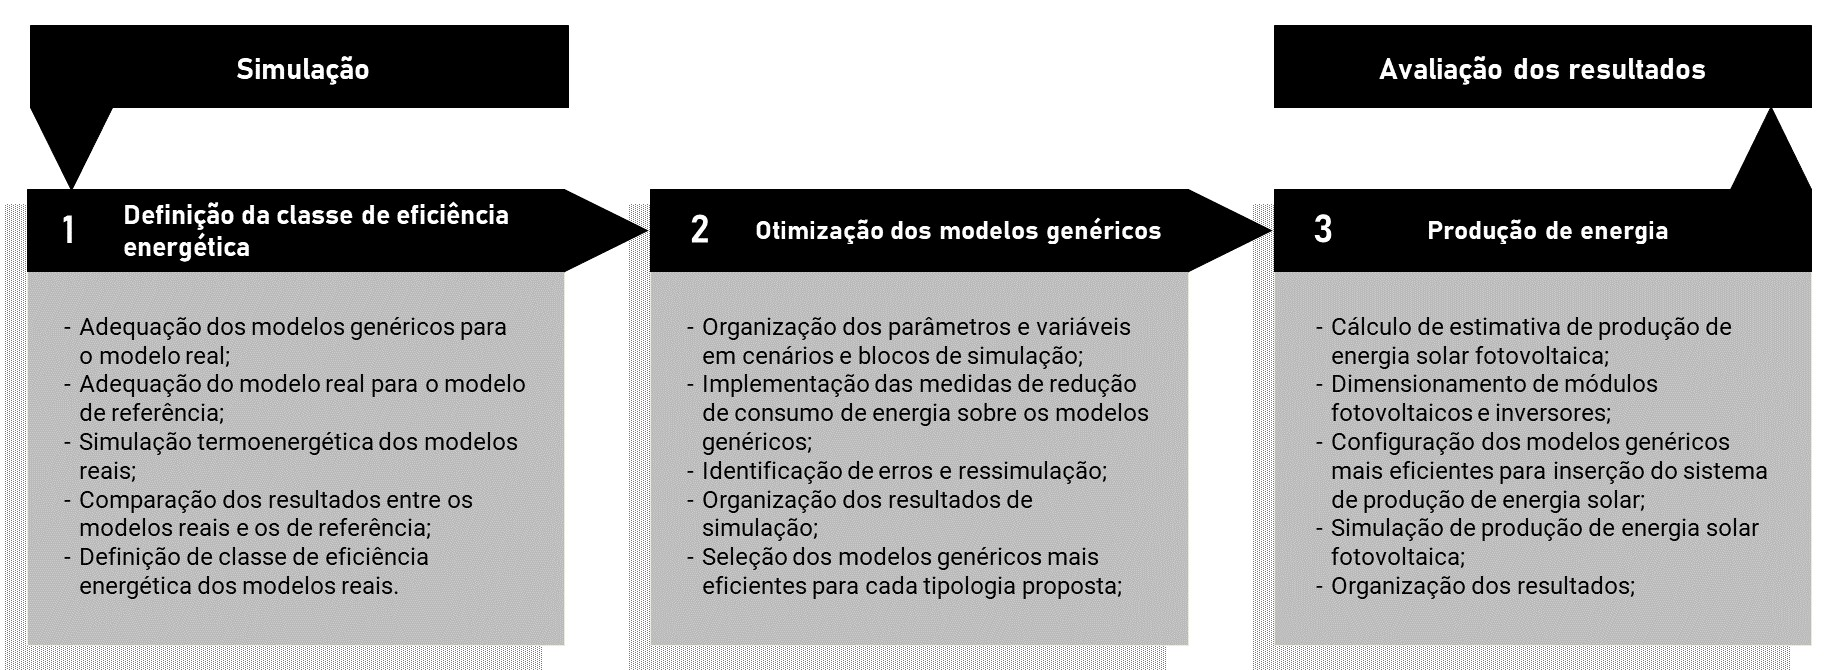
\includegraphics[width=1.0\textwidth]{figures/fig14-fluxograma-3.jpg}
    \begin{flushleft}
        \par \small Fonte: autor (2019)
    \end{flushleft}
    \label{fig:figura14}
\end{figure}
\subsubsection{Processo de modelagem}
\noindent Na etapa de modelagem foi realizada a composição dos modelos genéricos utilizando ferramentas computacionais de simulação de eficiência energética. Nesta fase foram configurados e ajustados os parâmetros incorporados aos modelos, como as características volumétricas, dados de desempenho dos equipamentos e soluções arquitetônicas.\vspace*{0.3cm} \newline
\noindent Trabalhos como o de Didoné \citeyear{Didone2014}, que realizou um estudo paramétrico de estratégias para edificações com balanço energético nulo no Brasil, utilizou o \textit{EnergyPlus} como principal ferramenta para simulação dos cenários termoenergéticos propostos. Carlo \citeyear{Carlo2008}, que desenvolveu uma metodologia de avaliação da eficiência energética para a envoltória de edificações não-residenciais, também utilizou essa ferramenta por reunir funções que auxiliariam na simulação de desempenho termoenergético e de parâmetros econômicos para verificação do consumo energético do modelo proposto.\vspace*{0.3cm} \newline
\noindent Outros autores aplicam o EnergyPlus por ser um software open source ou seja, software livre, amplamente utilizado pela comunidade cientifica e por reduzir os esforços no desenvolvimento de modelos matemáticos complexos para simulação de cenários termoenergéticos, auxiliando na otimização energética dos modelos propostos em estudo \cite{Vuong2015,Dahanayake2017,Shen2018,Kamal2019}.\vspace*{0.3cm} \newline
\noindent Portanto, a escolha da ferramenta mais apropriada para a modelagem dos parâmetros escolhidos como recurso ao processo de simulação da metodologia foi necessária. Seguindo a premissa de que a ferramenta deveria ser de livre acesso, ser validada em âmbito acadêmico e apresentar o maior volume de utilização em estudos de caso possível, como exemplificado na Figura \ref{fig:figure15}, foi adotado o software de simulação de energia em edificações \textit{EnergyPlus} 9.1.0-08d2e308bb \cite{U.S.DepartmentofEnergy-USDOE2011,Athienitis2015}.\vspace*{0.3cm} \newline
\noindent Da mesma forma, segundo Brackney et al. \citeyear{Brackney2018}, para facilitar o processo de configuração volumétrica e energética dos modelos, foram utilizadas ferramentas de suporte, que forneceram a interface entre o simulador e a ferramenta de modelagem. Estas ferramentas foram o \textit{SketchUp} 2017 trial version, versão 17.0.18899 \cite{TrimbleInc.2019}, para modelagem computacional tridimensional do edifício, e as extensões open-source para \textit{SketchUp, OpenStudio} v2.8.0, e a ferramenta de análise paramétrica \textit{Parametric Analysis Tool} – PAT.\vspace*{0.3cm} \newline
\begin{figure}[H]
    \centering
    \caption{\textit{Softwares} mais utilizados em simulação de eficiência de edificações.}
    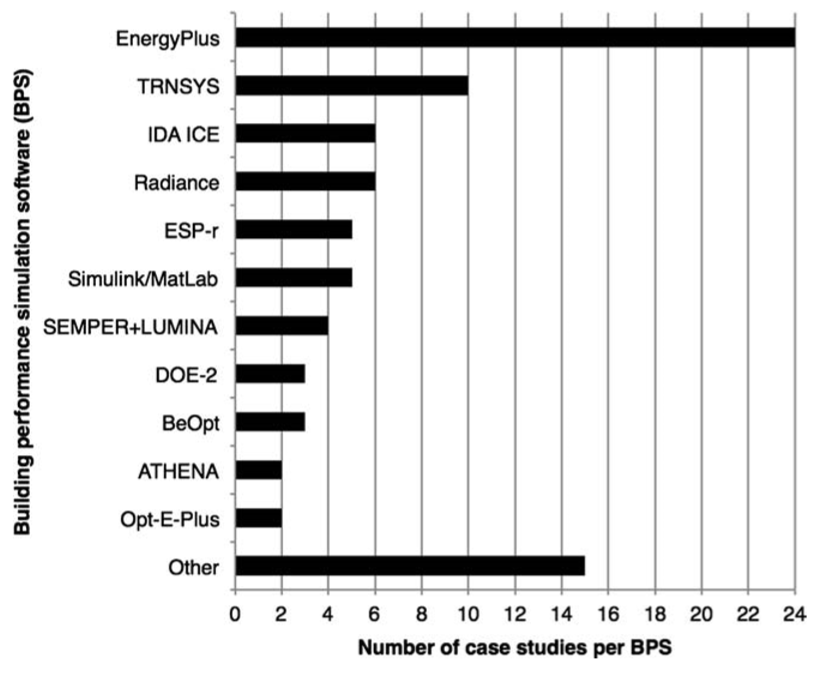
\includegraphics[width=0.8\textwidth]{figures/fig15-grafico-soft.png}
    \begin{flushleft}
        \par \small Fonte: adaptado de Athienitis; O’Brien (2015, tradução nossa).
    \end{flushleft}
    \label{fig:figure15}
\end{figure}
\noindent O início do processo de modelagem se dá pela configuração da volumetria utilizando as ferramentas internas do software de simulação computacional. Foram criadas as zonas térmicas das torres e dos pavimentos térreo e garagens, dimensões de aberturas externas e internas de cada zonas, assim como a quantidade de pavimentos-tipo das torres de cada modelo, definições de superfícies como piso, paredes e teto, e as áreas comuns de circulação horizontal e vertical, como ilustrado na Figura \ref{fig:figure16}.\vspace*{0.3cm} \newline
\noindent As janelas foram dimensionadas com cerca de 50\% do PAF\textsubscript{T}, com tamanhos variados, e com infiltração de ar padrão de 0,0003 m³/h/m² de área externa, como previamente definido na composição dos modelos genéricos. Todavia, as portas foram inseridas com medidas padrão reunidas em levantamento. Estas foram modeladas de acordo com as dimensões mais frequentes observadas no levantamento realizado, com 0,70 metros por 2,10 metros, e com infiltração de ar padrão da ferramenta de 0,0003 m³/h/m² de área de piso interna.\vspace*{0.3cm} \newline
\noindent Concluída a configuração da volumetria, inicia-se a composição dos dados do sítio onde o modelo genérico está implantado. Assim, foi inserido o arquivo climático de Vitória com os dados climáticos de 2018, no formato \textit{EnergyPlus Weather} – EPW, juntamente aos dias úteis do ano selecionado, no formato \textit{Design Conditions Design Days Data} – DDY \cite{InstitutoNacionaldeMetereologia-INMET2018}. Da mesma forma, foram configurados os dados da zona climática definida pela ASHRAE, 1A, similar à zona climática do recorte territorial.\vspace*{-0.25cm}
\begin{figure}[H]
    \centering
    \caption{Interface de configuração dos modelos genéricos no \textit{plug-in OpenStudio}.}
    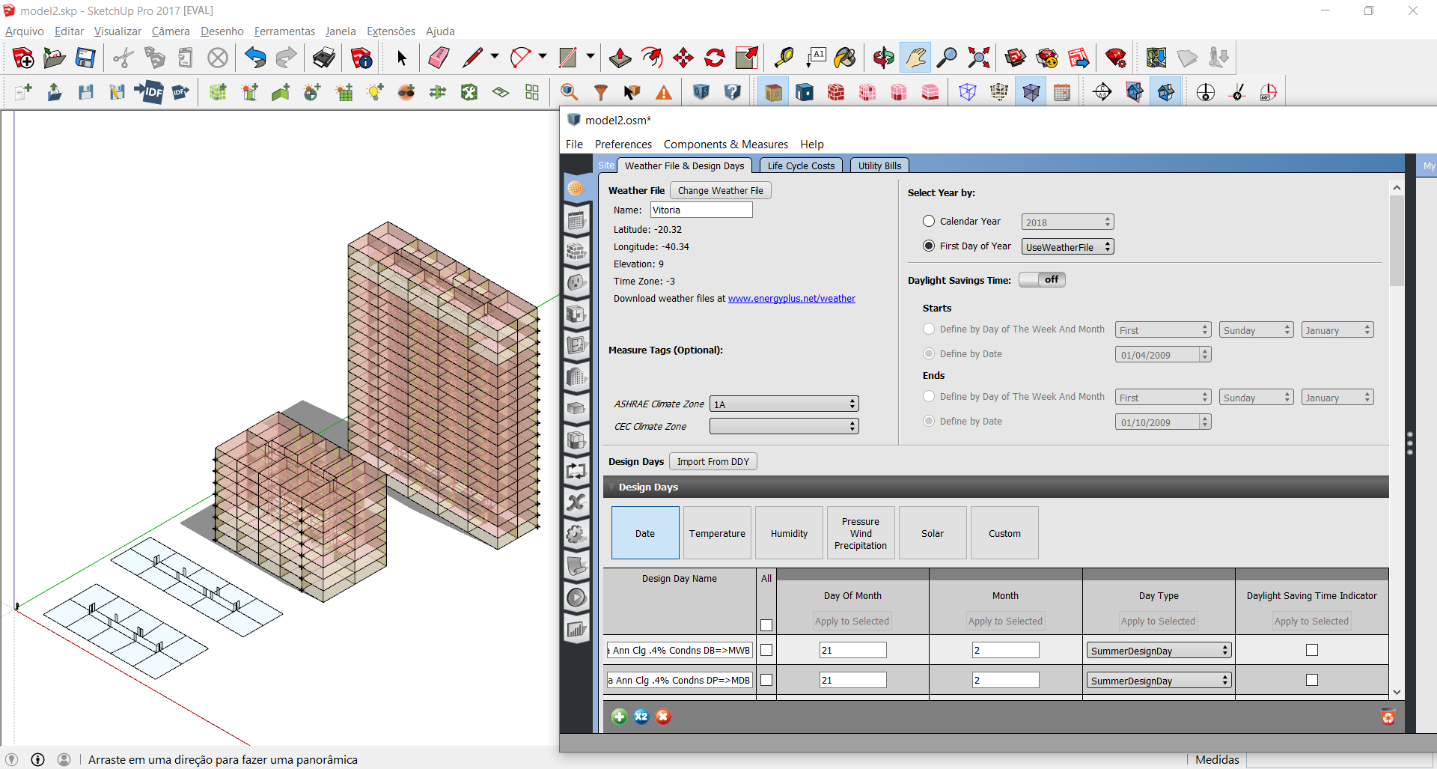
\includegraphics[width=0.8\textwidth]{figures/fig16-OS.png}
    \begin{flushleft}
        \par \small Fonte: autor, (2019).
    \end{flushleft}
    \label{fig:figure16}
\end{figure}
\noindent Concluída a etapa de geometrização e modelagem tridimensional da edificação, é dado início às configurações da envoltória, onde são atribuídos os dados de entrada característicos do empreendimento, como os valores de propriedades térmicas dos elementos construtivos, os dados de ocupação, por meio de schedules para vestimenta, horários de utilização dos ambientes, aberturas, iluminação e equipamentos, como exemplificado na Figura \ref{fig:figure17}.\vspace*{-0.25cm}
\begin{figure}[H]
    \centering
    \caption{Colagem da interface de inserção de dados das propriedades térmicas e de materiais.}
    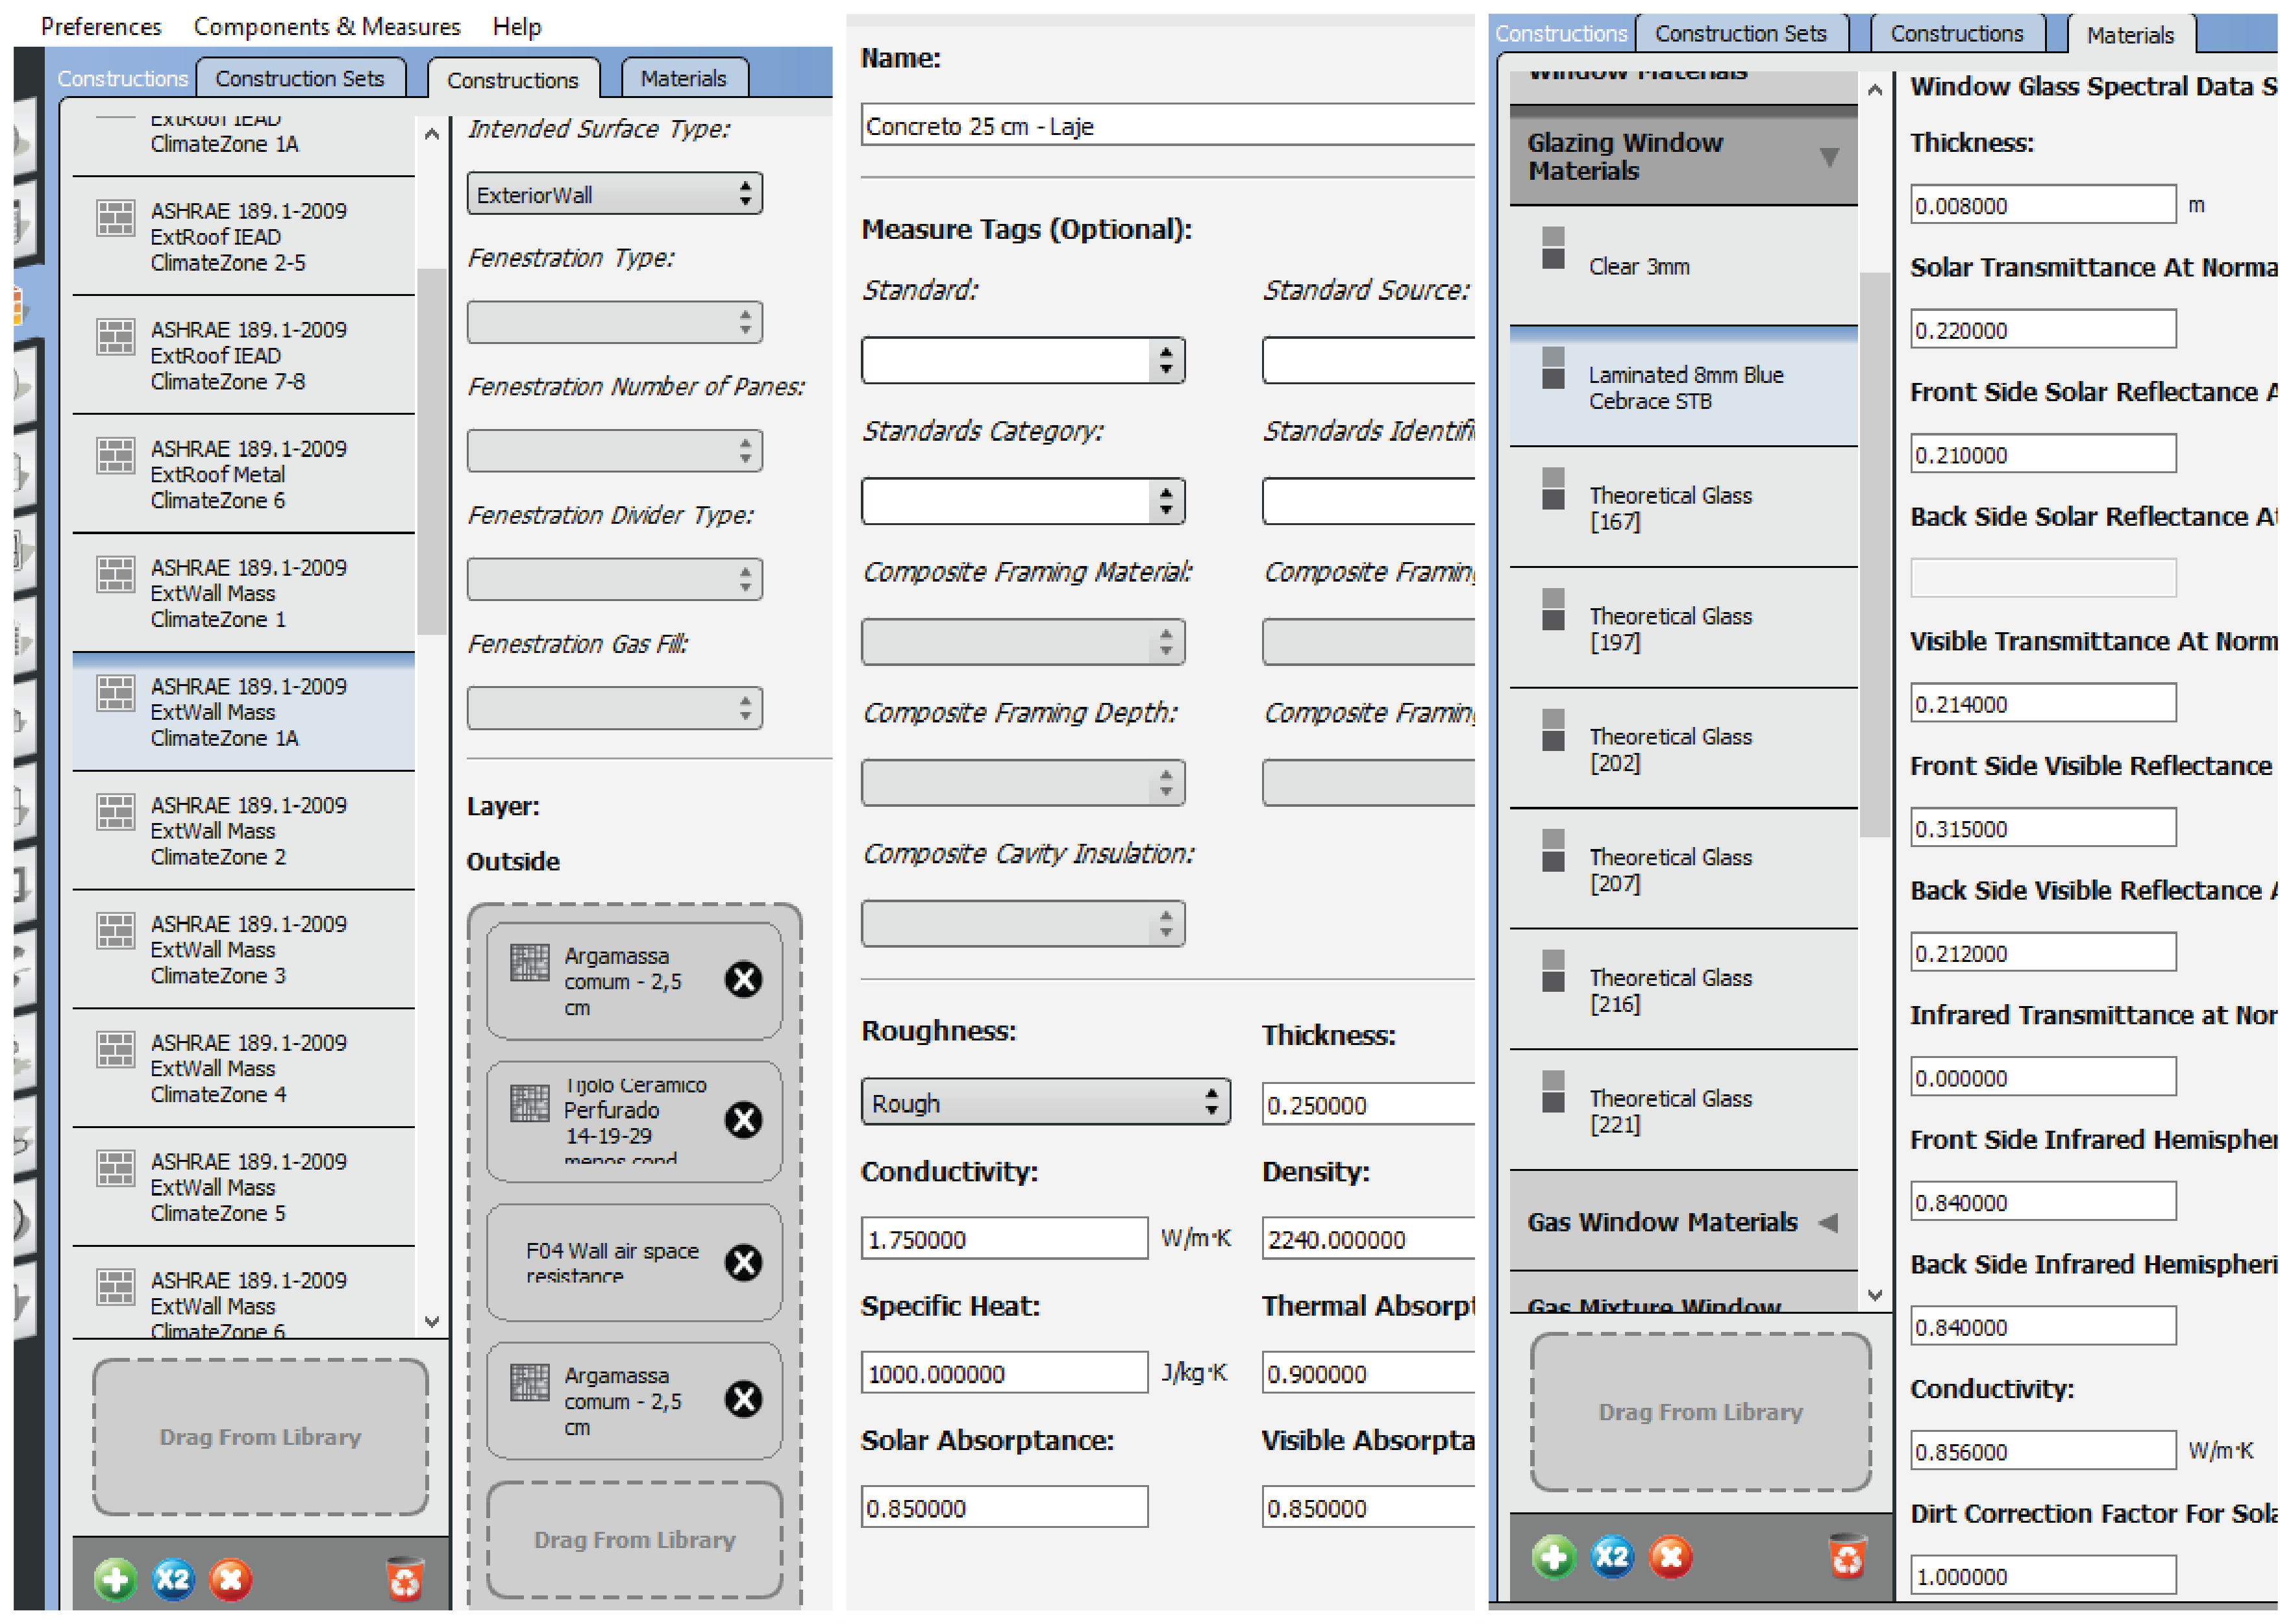
\includegraphics[width=0.8\textwidth]{figures/fig17-OS2.png}
    \begin{flushleft}
        \par \small Fonte: autor, (2019).
    \end{flushleft}
    \label{fig:figure17}
\end{figure}
\noindent Em seguida, foram configurados o sistema de condicionamento de ar, apresentado pela Figura \ref{fig:figure18}, segundo as características definidas para os modelos genéricos. Da mesma forma, foram implementadas medidas de parametrização das variáveis, medidas estas denominadas \textit{measures}, com a finalidade de reduzir o tempo total de processamento e simulação dos cenários. As \textit{measures} adotadas parametrizaram as mudanças de orientação solar, de componentes construtivos, de equipamentos de ar-condicionado e redução de carga de energia.\vspace*{-0.25cm}
\begin{figure}[H]
    \centering
    \caption{Interface de configuração dos sistemas de condicionamento de ar.}
    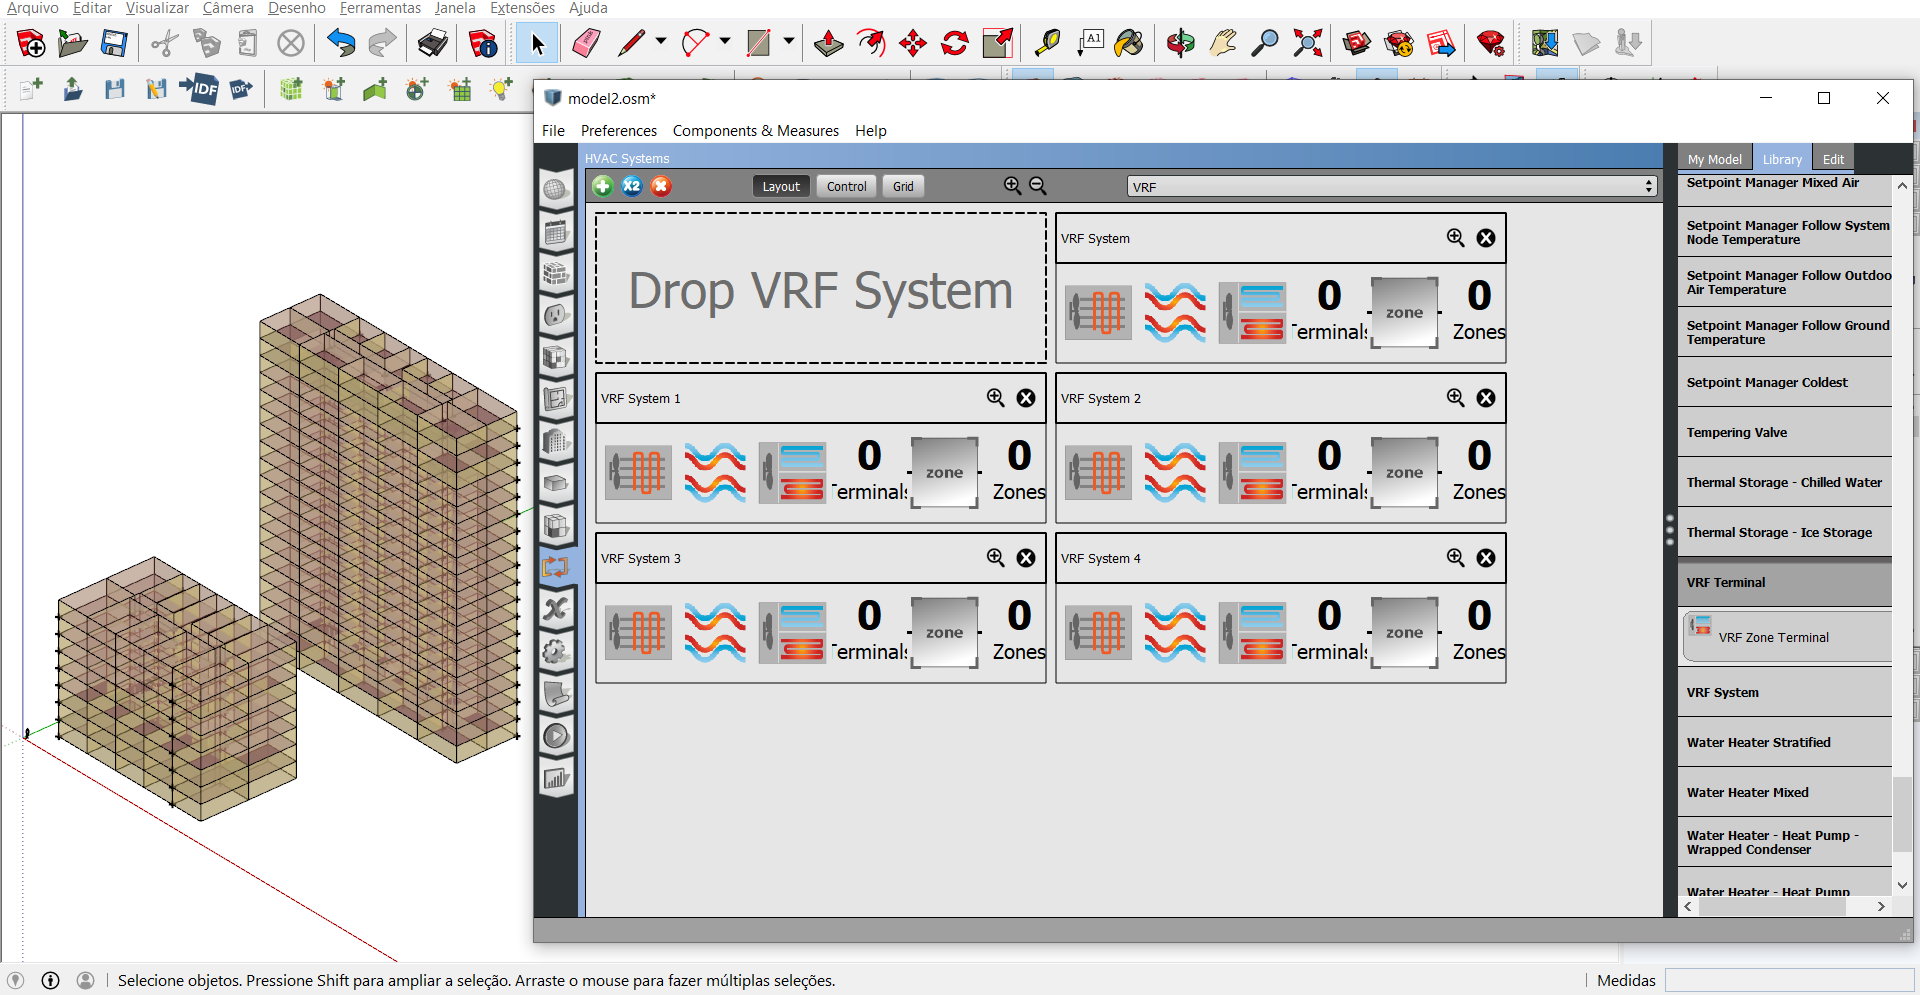
\includegraphics[width=0.85\textwidth]{figures/fig18-OS3.png}
    \begin{flushleft}
        \par \small Fonte: autor, (2019).
    \end{flushleft}
    \label{fig:figure18}
\end{figure}
\noindent Após as configurações de envoltória e sistemas concluídas, foram selecionadas as variáveis de saída relevantes à análise e feito a simulação teste, como exemplificado na Figura \ref{fig:figure19}. Desta forma os resultados foram concentrados nos dados de saída mais pertinentes, reduzindo o tempo total de simulação. Posteriormente, os modelos foram simplificados geometricamente, utilizando o recurso multiply, como abordado no subcapitulo sobre simplificação dos modelos genéricos \cite{Brackney2018}.\newline
\begin{figure}[H]
    \centering
    \caption{Saídas da simulaçãoem processo de finalização.}
    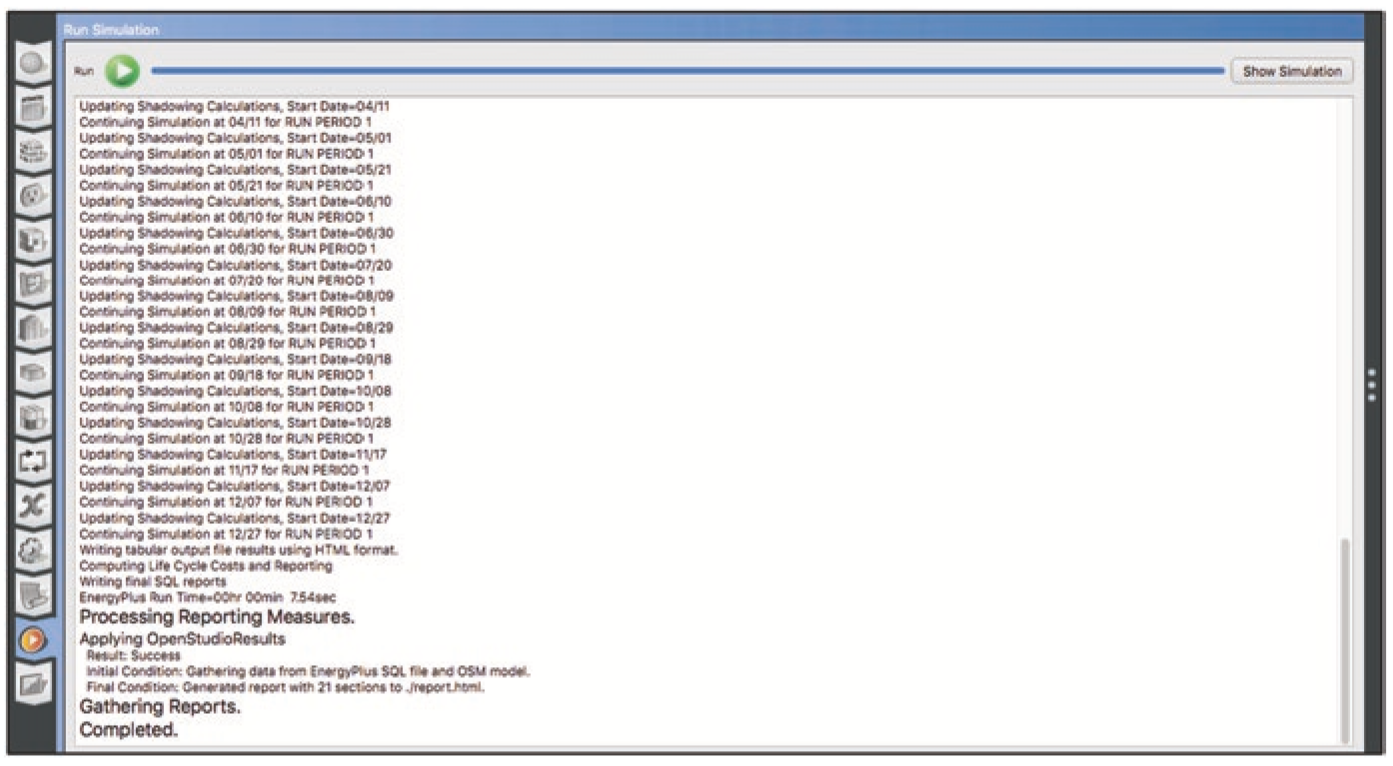
\includegraphics[width=0.9\textwidth]{figures/fig19-OS4.png}
    \begin{flushleft}
        \par \small Fonte: adaptado de Brackney et al. (2018).
    \end{flushleft}
    \label{fig:figure19}
\end{figure}
\subsubsection{Simplificação dos modelos genéricos e parametrização dos cenários}
\noindent A simulação energética e análise de um único cenário requer a utilização da ferramenta básica de modelagem, construção e revisão, que neste caso foi a ferramenta \textit{OpenStudio}. Entretanto, como este trabalho analisa vários cenários pertinentes a mais do que um modelo, foi necessária uma ferramenta mais robusta, que proporcionasse simulações simultâneas dos cenários construídos. Para esta finalidade, a ferramenta de parametrização PAT foi utilizada.\vspace*{0.3cm} \newline
\noindent Entretanto, um requisito necessário para que as simulações ocorram de forma simultânea e consumam pouco tempo de recurso computacional é a simplificação dos modelos. Esta simplificação consiste em reduzir o número de zonas térmicas a serem simuladas por meio da subtração de pavimentos que não sofrem influência da radiação solar e intempéries em uma edificação.\vspace*{0.3cm} \newline
\noindent Diante do exposto, o primeiro e o ultimo pavimento, juntamente ao pavimento intermediário a eles, foram mantidos, como apresentado na Figura \ref{fig:figure20}. Este recurso de redução de tempo de simulação é possível utilizando a função multiply disponibilizado pelo \textit{EnergyPlus} \cite{U.S.DepartmentofEnergy-USDOE2019}. Esta função tem como característica replicar os pavimentos selecionados a fim de multiplicar o número de zonas térmicas, área de piso e energia consumida pela carga interna virtualmente, substituindo as zonas térmicas modeladas e excluídas anteriormente.\newline
\begin{figure}[H]
    \caption{Modelos genéricos simplificados.}
    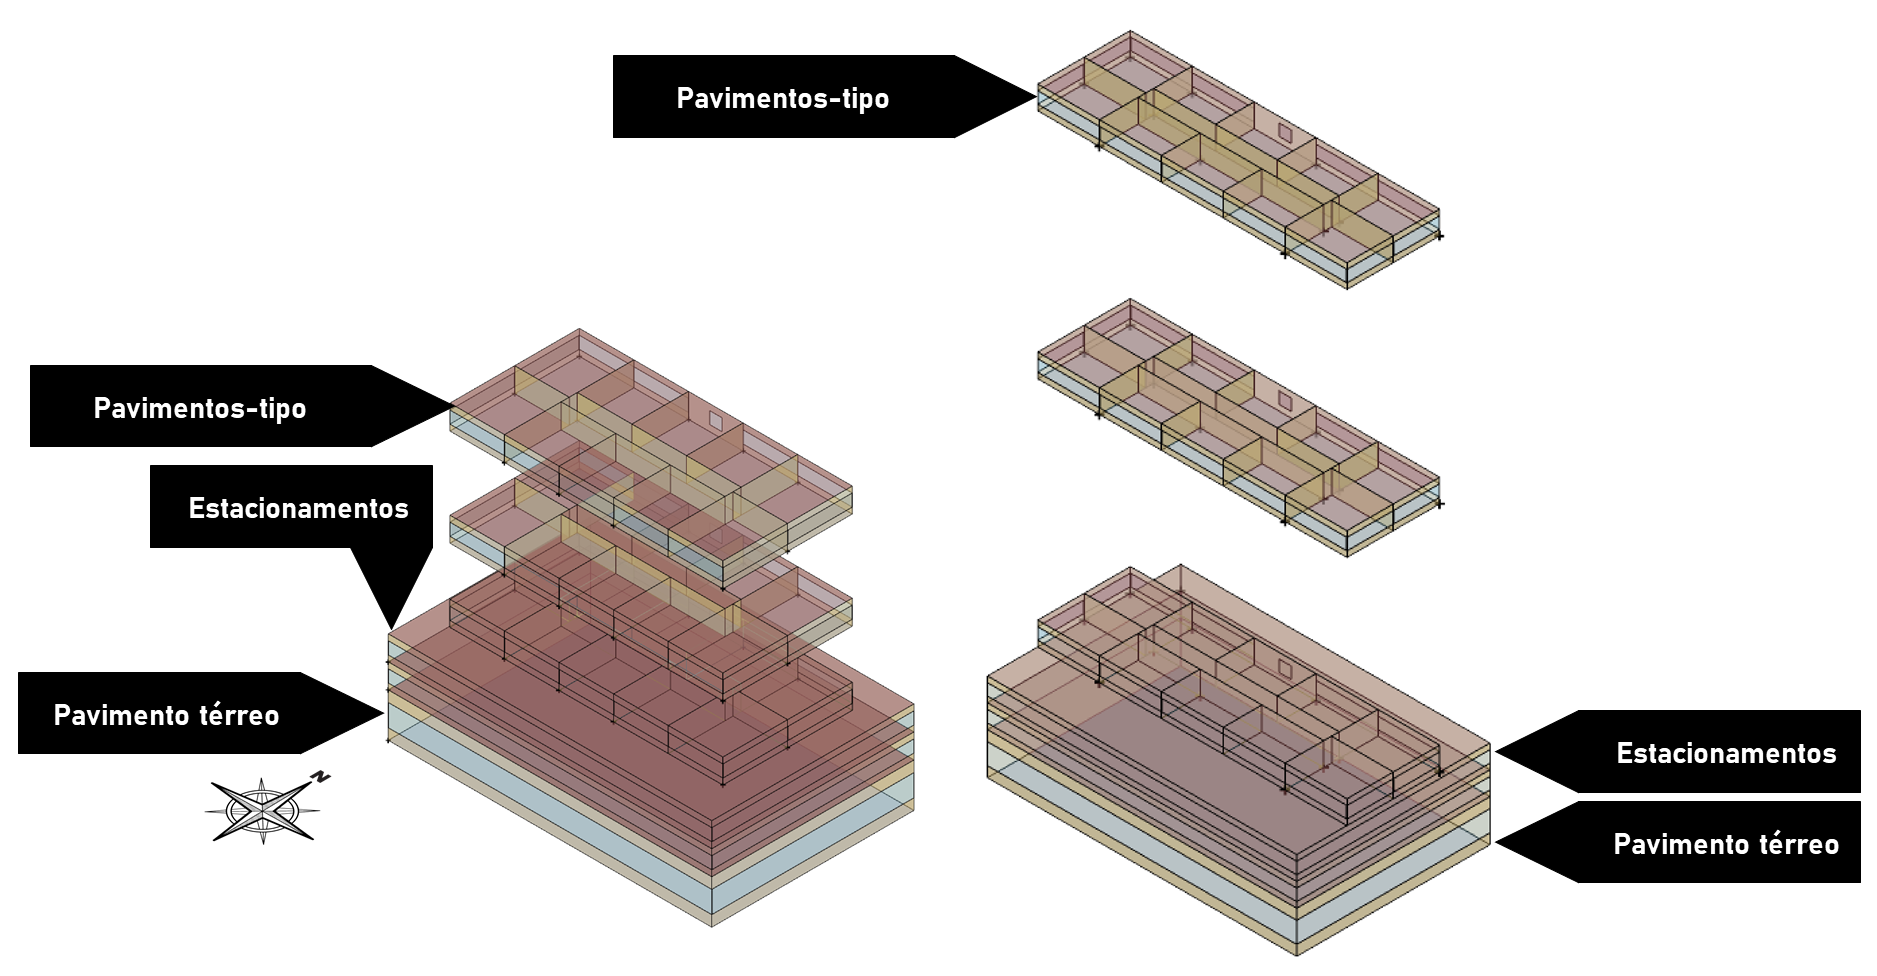
\includegraphics[width=1.0\textwidth]{figures/fig20-modelos.png}
    \begin{flushleft}
        \par \small Fonte: autor, (2019).
    \end{flushleft}
    \label{fig:figure20}
\end{figure}
\noindent Assim, a partir dos modelos simplificados, foram configurados os 368 cenários utilizando a ferramenta PAT, processo ilustrado pela Figura \ref{fig:figure21}. Desta forma, estes cenários que abrangem a etapa de otimização dos modelos genéricos foram simulados simultaneamente, reduzindo o tempo total de simulação e obtenção de resultados.\newline
\begin{figure}[H]
    \caption{Interface do \textit{Parametric Analysis Tool.}}
    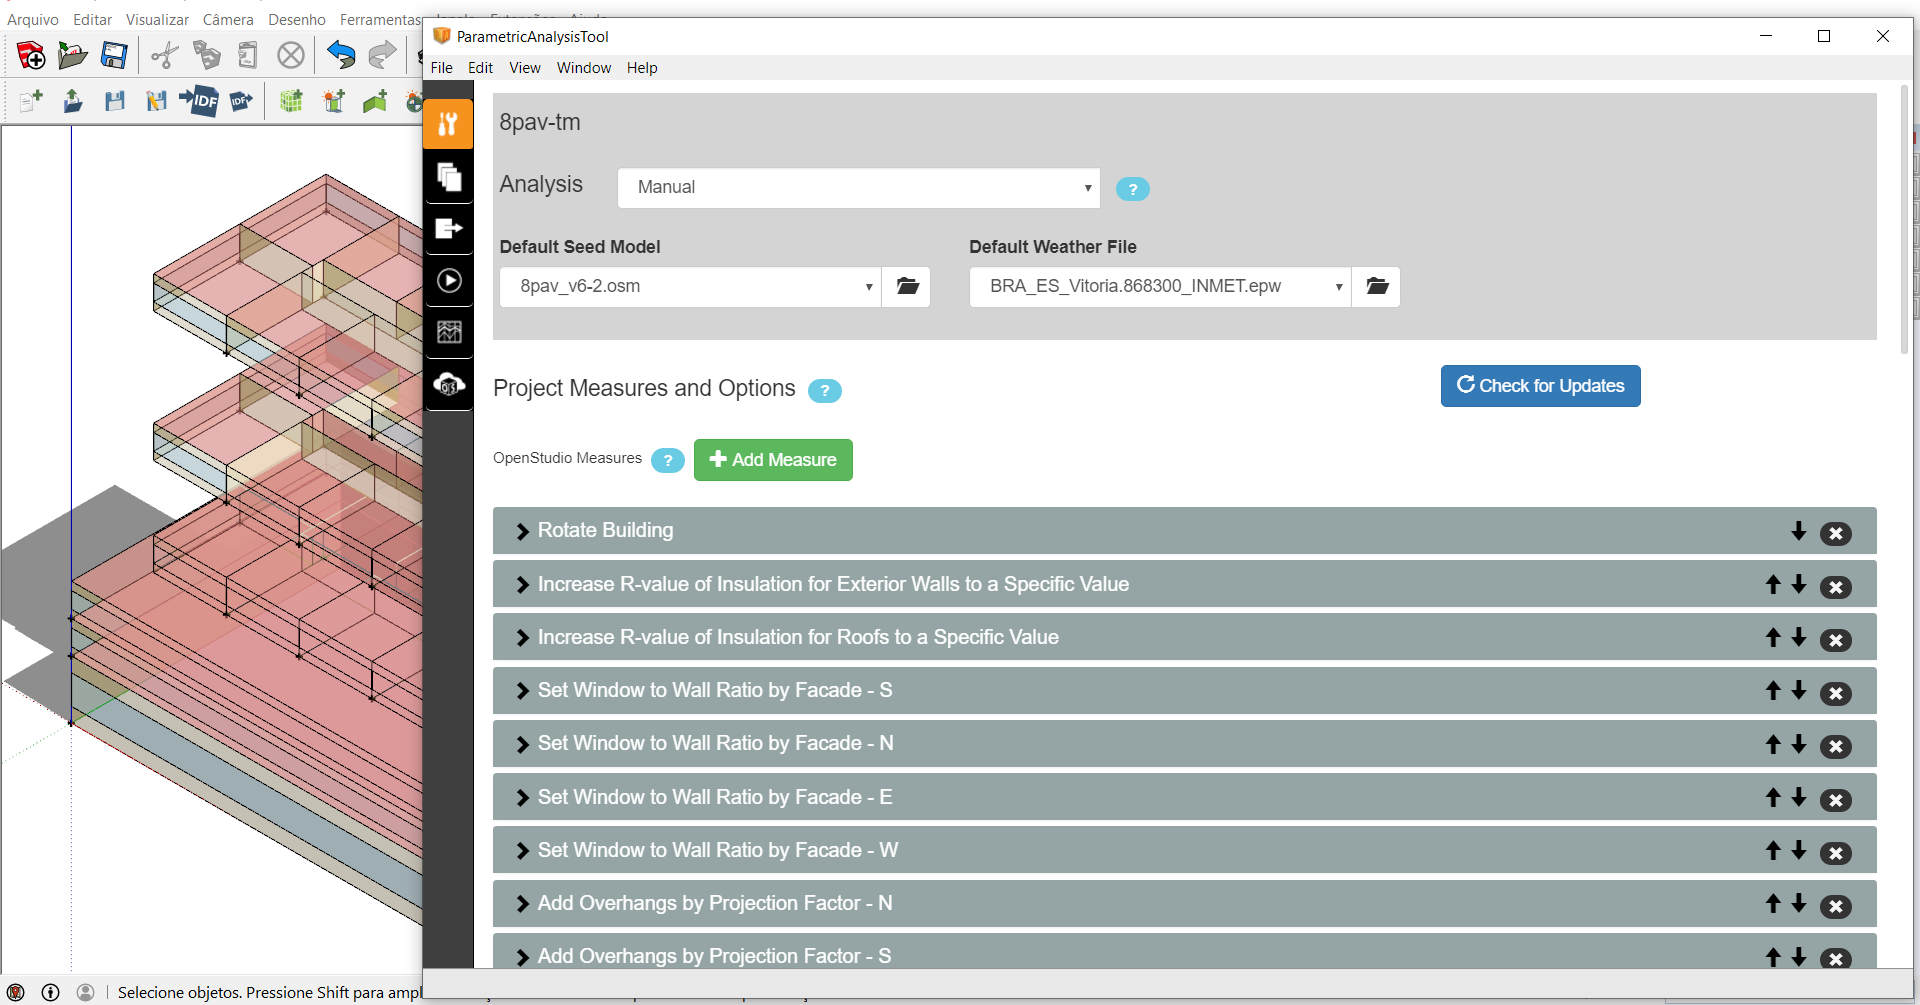
\includegraphics[width=1.0\textwidth]{figures/fig21-modelos.png}
    \begin{flushleft}
        \par \small Fonte: autor, (2019).
    \end{flushleft}
    \label{fig:figure21}
\end{figure}
\subsubsection{Processo de modelagem}
\noindent A partir da etapa de otimização, as informações reunidas sobre as estratégias passivas e ativas utilizadas neste trabalho serviram como base de dados para a configuração das measures no processo de simulações da PAT. As measures de estratégias ativas, como as medidas substituição do sistema de condicionamento de ar e de redução de carga de energia elétrica, foram executadas, respectivamente, no primeiro e no último bloco de simulações, compreendendo as reduções ativas de Intensidade de Uso de Energia e consumo final energético.\vspace*{0.3cm} \newline
\noindent Concomitantemente, os blocos de simulação implementados entre as medidas ativas de redução de energia englobaram as estratégias passivas, como mudança de PAF\textsubscript{T}, de componentes construtivos e alterações volumétricas e de orientação solar das fachadas. O processo de simulação dos cenários obedeceu a sequência de implementação das medidas para redução de consumo de energia disposta na Tabela \ref{tab:tabela13}.\vspace*{-0.1cm}
\begin{table}[H]
    \small
    \caption{\textit{Measures} utilizadas e os parâmetros correlacionados.}
    \begin{tabular}{llll}
    \hline
    \multicolumn{1}{c}{\textit{\textbf{Measure}}}                                                                                        & \multicolumn{1}{c}{\textbf{Parâmetro alvo}}                                                       & \multicolumn{2}{c}{\textbf{Inputs}}  \\ \hline
    \multirow{3}{*}{\makecell[l]{\textit{ZEGD VRF with DOAS;} \\ \textit{Add aPSZ-HP to each zone}}}                            & \multirow{3}{*}{\makecell[l]{Sistema de Condicionamento \\de Ar}}                                                 & a  & \textit{CAG/Fancoil}            \\
                                                                                                                                &                                                                                                   & b  & \textit{Split}                  \\
                                                                                                                                &                                                                                                   & c  & VRF                             \\ \hline
    \multicolumn{1}{l}{\multirow{4}{*}{\textit{Rotate Building}}}                                                               & \multicolumn{1}{l}{\multirow{4}{*}{Orientação solar}}                                             & a  & 0°                              \\
    \multicolumn{1}{l}{}                                                                                                        & \multicolumn{1}{l}{}                                                                              & b  & 90°                             \\
    \multicolumn{1}{l}{}                                                                                                        & \multicolumn{1}{l}{}                                                                              & c  & 180°                            \\
    \multicolumn{1}{l}{}                                                                                                        & \multicolumn{1}{l}{}                                                                              & d  & 270°                            \\ \hline
    \multirow{3}{*}{\makecell[l]{\textit{Increase R-value of Insulation for} \\ \textit{Exterior Walls to a Specific Value}}}   & \multirow{3}{*}{\makecell[l]{Transmitância térmica \\da parede da envoltória}}                    & a  & 2,46 W/m²K                      \\
                                                                                                                                &                                                                                                   & b  & 0,38 W/m²K                      \\
                                                                                                                                &                                                                                                   & c  & 0,32 W/m²K                      \\ \hline
    \multirow{3}{*}{\makecell[l]{\textit{Increase R-value of Insulation for} \\ \textit{Roofs to a Specific Value}}}            & \multirow{3}{*}{\makecell[l]{Transmitância térmica da \\cobertura}}                                               & a  & 3,73 W/m²K                      \\
                                                                                                                                &                                                                                                   & b  & 0,55 W/m²K                      \\
                                                                                                                                &                                                                                                   & c  & 0,53 W/m²K                      \\ \hline
    \multirow{3}{*}{\textit{Set Window to Wall Ratio by Facade}}                                                                & \multirow{3}{*}{\makecell[l]{Percentual de Área de \\Abertura da Fachada Total}}                  & a  & 30\%                            \\
                                                                                                                                &                                                                                                   & b  & 50\%                            \\
                                                                                                                                &                                                                                                   & c  & 80\%                            \\ \hline
    \multirow{3}{*}{\textit{Add overhangs by Projection Factor}}                                                                & \multirow{3}{*}{Proteção solar}                                                                   & a  & 20 cm                           \\
                                                                                                                                &                                                                                                   & b  & 50 cm                           \\
                                                                                                                                &                                                                                                   & c  & 100 cm                          \\ \hline
    \multirow{2}{*}{\textit{Reduce Lighting Loads by Percentage}}                                                               & \multirow{2}{*}{\makecell[l]{Medidas de Redução de Carga\\ de Energia Elétrica: Iluminação}}      & a  & n/a                             \\
                                                                                                                                &                                                                                                   & b  & 30\%                            \\ \hline
    \multirow{2}{*}{\textit{Reduce Equipment Loads by Percentage}}                                                              & \multirow{2}{*}{\makecell[l]{Medidas de Redução de Carga\\ de Energia Elétrica: Equipamentos}}    & a  & n/a                             \\
                                                                                                                                &                                                                                                   & b  & 30\%                            \\ \hline
    \multirow{2}{*}{\textit{Add, Remove or Replace Window}}                                                                     & \multirow{2}{*}{\makecell[l]{Vidros com transmitância \\térmica baixa}}                                           & a  & 0,44 W/m²K                      \\
                                                                                                                                &                                                                                                   & b  & 0,16 W/m²K                      \\ \hline
    \end{tabular}
    \begin{flushleft}
        \par \small Fonte: autor (2019).
    \end{flushleft}
    \label{tab:tabela13}
\end{table}
\vspace{-0.60cm} \noindent Com estas medidas, buscou-se atingir a eficiência energética necessária para o balanço energético dos modelos propostos, complementando a economia com produção de energia de fontes renováveis.

\subsubsection{Estimativa de produção de energia}
\noindent Para esta pesquisa, foi aplicado o sistema de produção de energia fotovoltaica, tanto por ser a mais usual nesse tipo de edificação como, também, pela complexidade da análise de custos para os outros sistemas, que inviabilizaria a conclusão da avaliação dentro do tempo disponível para o desenvolvimento do trabalho.\vspace*{0.3cm} \newline
\noindent A geração de energia solar foi avaliada a partir da área disponível para a implantação dos painéis fotovoltaicos. A área considerada para a produção de energia é constituída pela área de cobertura, de estacionamento, áreas opacas das fachadas e das proteções solares \cite{Didone2014}. Assim como a verificação de disponibilidade de áreas, os dados sobre a irradiação solar, radiação global difusa e anual, e a temperatura média anual de Vitória, extraídos do arquivo climático da cidade, foram considerados para a estimativa de produção de energia \cite{InstitutoNacionaldeMetereologia-INMET2018,Pereira2017}.\vspace*{0.3cm} \newline
\noindent A estimativa de produção de energia solar foi calculada com base no estudo de Palaoro \citeyear{Palaoro2019} sobre dimensionamento de sistema  fotovoltaico. Esta estimativa, necessária para suprir a demanda energética das edificações propostas, foi essencial para a obtenção  de dados para a simulação computacional de geração de energia solar fotovoltaica.\vspace*{0.3cm} \newline
\noindent Inicialmente foi calculada a energia de geração, E\textsubscript{geração}, como exposto na Equação \ref{eq:eq3}.
\begin{equation}\label{eq:eq3}
E_{geracao}=\frac{V_m}{30}
\end{equation}
\noindent Onde:\par
\setlength\parindent{1.5cm} E\textsubscript{geração} representa a quantidade de energia de geração, em kWh/mês; e\par
\setlength\parindent{1.5cm} V\textsubscript{m} é o valor médio de consumo da edificação.\par
\noindent Uma vez conhecida a energia de geração, foi estimada a quantidade de energia que cada modulo produziria diariamente, E\textsubscript{m}. De acordo com a Equação \ref{eq:eq4}, tem-se:
\begin{equation}\label{eq:eq4}
E_m=E_s \times A_m \times {\eta}_m
\end{equation}
\noindent Onde:\par
\setlength\parindent{1.5cm} E\textsubscript{m} é a quantidade estimada de energia produzida pelo modulo, expressa em Wh/dia;\par
\setlength\parindent{1.5cm} E\textsubscript{s} é a irradiação solar, em Wh/m²/dia;\par
\setlength\parindent{1.5cm} A\textsubscript{m} compreende a área da superfície do modulo, em m²; e\par
\setlength\parindent{1.5cm} \(\eta\)\textsubscript{m} é a eficiência do módulo.\par
\noindent Com as estimativas de geração de energia geral e por cada modulo diariamente, foram calculadas a  quantidade  de  módulos  necessários  para  atender  a  estimativa  de  geração  de  energia.  A quantidade de módulos, N\textsubscript{m}, é resultado da razão entre a quantidade de energia gerada, E\textsubscript{geração}, sobre a quantidade de energia gerada por cada modulo individualmente, E\textsubscript{m}. Desta forma, como expresso pela Equação \ref{eq:eq5}, tem-se que:
\begin{equation}\label{eq:eq5}
N_m=\frac{E_{geracao}}{E_m}
\end{equation}
\noindent Os módulos e inversores foram pesquisados de acordo com as dimensões e especificações estimadas por meio das equações demonstradas neste capítulo, como apresentado na Tabela \ref{tab:tabela14}. O sistema fotovoltaico indicado ao cenário dos modelos genéricos foi de porte comerciais, dada a demanda de energia calculada. Os inversores foram dimensionados de forma a aproveitar a potência máxima nominal dos módulos, evitando o subdimensionamento e inadequação entre inversores e módulos durante o processo de geração de energia do sistema fotovoltaico.
\subsubsection{Simulação de geração de energia}
\noindent A simulação de produção de energia solar foi realizada por meio da ferramenta PVsyst, versão v6.8.1 \cite{Cronemberger2012}. Esta ferramenta foi utilizada por disponibilizar a análise de desempenho e dimensionamento do sistema de produção de energia solar necessário para empreendimentos do porte da edificação proposta nesta pesquisa. Complementarmente a ferramenta, foi feito um levantamento dos módulos fotovoltaicos comercializados no Brasil de acordo com a aplicação destes componentes sobre a envoltória, como módulos monocristalinos de silício, m-Si, e filme fino de Telúrio de Cádmio, Cd-Te \cite{Didone2014,Werneck2017,Sorgato2018}. Estas tecnologias foram escolhidas por serem indicadas para a aplicação sobre as superfícies horizontais, como a cobertura e o estacionamento, e verticais, como as fachadas.\newline
\begin{table}[H]
    \small
    \caption{Módulos fotovoltaicos utilizados e a áreadisponível para implantação.}
    \begin{tabular}{lllll}
    \hline
    \multicolumn{2}{c}{\multirow{2}{*}{\textbf{Características}}}                                                                                   & \multicolumn{3}{c}{\textbf{Modelo genérico de 8 pavimentos}}                                                                                                                   \\ \cline{3-5} 
    \multicolumn{2}{c}{}                                                                                                                            & \multicolumn{1}{c}{\makecell[c]{\textbf{Cobertura} \\\textbf{e estacionamento}}}   & \multicolumn{1}{c}{\makecell[c]{\textbf{Proteção} \\ \textbf{solar}}}            & \multicolumn{1}{c}{\textbf{Fachada}}                      \\ \hline
    \multicolumn{1}{c}{\parbox[t]{2mm}{\multirow{8}{*}{\rotatebox[origin=c]{90}{\textbf{Módulo}}}}} & Módulo                                        & \multicolumn{1}{c}{\makecell[c]{SunPower \\SPR-E20-435-COM}}              & \multicolumn{1}{c}{\makecell[c]{SunPower \\SPR-E20-435-COM}}           & \multicolumn{1}{c}{\makecell[c]{First Solar \\FS-4122-2}}                 \\
    \multicolumn{1}{c}{}                                                                            & Tecnologia                                    & \multicolumn{1}{c}{m-SI}                                  & \multicolumn{1}{c}{m-SI}                               & \multicolumn{1}{c}{Cd-Te}                                 \\
    \multicolumn{1}{c}{}                                                                            & Potência máx. (Wp)                            & \multicolumn{1}{c}{435}                                   & \multicolumn{1}{c}{435}                                & \multicolumn{1}{c}{122,5}                                 \\
    \multicolumn{1}{c}{}                                                                            & Tensão máx. (V)                               & \multicolumn{1}{c}{324}                                   & \multicolumn{1}{c}{648}                                & \multicolumn{1}{c}{376}                                   \\
    \multicolumn{1}{c}{}                                                                            & \makecell[l]{Potência Nominal \\- STC (kWp)}  & \multicolumn{1}{c}{150}                                   & \multicolumn{1}{c}{100,92}                             & \multicolumn{1}{c}{274,22}                                \\
    \multicolumn{1}{c}{}                                                                            & Nº de módulos                                 & \multicolumn{1}{c}{345}                                   & \multicolumn{1}{c}{232}                                & \multicolumn{1}{c}{2238}                                  \\
    \multicolumn{1}{c}{}                                                                            & Eficiência (\%)                               & \multicolumn{1}{c}{19}                                    & \multicolumn{1}{c}{19}                                 & \multicolumn{1}{c}{17}                                    \\
    \multicolumn{1}{c}{}                                                                            & Área ocupada (m²)                             & \multicolumn{1}{c}{746}                                   & \multicolumn{1}{c}{501}                                & \multicolumn{1}{c}{1612}                                  \\ \hline
    \parbox[t]{2mm}{\multirow{5}{*}{\rotatebox[origin=c]{90}{\textbf{Inversor}}}}                   & Modelo                                        & \multicolumn{1}{c}{\makecell[c]{Fronius \\International \\IG Plus 150 V-3}} & \multicolumn{1}{c}{\makecell[c]{Fronius \\International \\ECO 25.0-3-S}} & \multicolumn{1}{c}{\makecell[c]{Fronius International \\IG Plus 150 V-3}} \\
                                                                                                    & Nº de inversores                              & \multicolumn{1}{c}{10}                                    & \multicolumn{1}{c}{6}                                  & \multicolumn{1}{c}{14}                                    \\
                                                                                                    & \makecell[l]{Potência máx. \\total (kWac)}    & \multicolumn{1}{c}{120}                                   & \multicolumn{1}{c}{50}                                 & \multicolumn{1}{c}{84}                                    \\
                                                                                                    & Tensão de entrada (V)                         & \multicolumn{1}{c}{230-500}                               & \multicolumn{1}{c}{580-850}                            & \multicolumn{1}{c}{230-500}                               \\
                                                                                                    & Eficiência (\%)                               & \multicolumn{1}{c}{97,9}                                  & \multicolumn{1}{c}{97,9}                               & \multicolumn{1}{c}{97,9}                                  \\ \hline
    \multicolumn{2}{c}{\multirow{2}{*}{\textbf{Características}}}                                   & \multicolumn{3}{c}{\textbf{Modelo genérico de 19 pavimentos}}                                                                                                                   \\ \cline{3-5} 
    \multicolumn{2}{c}{}                                                                            & \multicolumn{1}{c}{\makecell[c]{\textbf{Cobertura} \\\textbf{e estacionamento}}}                          & \multicolumn{1}{c}{\makecell[c]{\textbf{Proteção} \\ \textbf{solar}}}            & \multicolumn{1}{c}{\textbf{Fachada}}                      \\ \hline
    \multicolumn{1}{c}{\parbox[t]{2mm}{\multirow{8}{*}{\rotatebox[origin=c]{90}{\textbf{Módulo}}}}} & Módulo                                        & \multicolumn{1}{c}{\makecell[c]{SunPower \\SPR-E20-435-COM}}              & \multicolumn{1}{c}{\makecell[c]{SunPower \\SPR-E20-435-COM}}           & \multicolumn{1}{c}{\makecell[c]{First Solar \\FS-4122-2}}                 \\
    \multicolumn{1}{c}{}                                                                            & Tecnologia                                    & \multicolumn{1}{c}{Si-mono}                                  & \multicolumn{1}{c}{Si-mono}                               & \multicolumn{1}{c}{Cd-Te}                                 \\
    \multicolumn{1}{c}{}                                                                            & Potência máx. (Wp)                            & \multicolumn{1}{c}{435}                                   & \multicolumn{1}{c}{435}                                & \multicolumn{1}{c}{122,5}                                 \\
    \multicolumn{1}{c}{}                                                                            & Tensão máx. (V)                               & \multicolumn{1}{c}{324}                                   & \multicolumn{1}{c}{648}                                & \multicolumn{1}{c}{376}                                   \\
    \multicolumn{1}{c}{}                                                                            & \makecell[l]{Potência Nominal \\- STC (kWp)}  & \multicolumn{1}{c}{150}                                   & \multicolumn{1}{c}{243,40}                             & \multicolumn{1}{c}{479,70}                                \\
    \multicolumn{1}{c}{}                                                                            & Nº de módulos                                 & \multicolumn{1}{c}{345}                                   & \multicolumn{1}{c}{560}                                & \multicolumn{1}{c}{3917}                                  \\
    \multicolumn{1}{c}{}                                                                            & Eficiência (\%)                               & \multicolumn{1}{c}{19}                                    & \multicolumn{1}{c}{19}                                 & \multicolumn{1}{c}{17}                                    \\
    \multicolumn{1}{c}{}                                                                            & Área ocupada (m²)                             & \multicolumn{1}{c}{746}                                   & \multicolumn{1}{c}{745}                                & \multicolumn{1}{c}{2820}                                  \\ \hline
    \parbox[t]{2mm}{\multirow{5}{*}{\rotatebox[origin=c]{90}{\textbf{Inversor}}}}                   & Modelo                                        & \multicolumn{1}{c}{\makecell[c]{Fronius \\International \\IG Plus 150 V-3}} & \multicolumn{1}{c}{\makecell[c]{Fronius \\International \\ECO 25.0-3-S}} & \multicolumn{1}{c}{\makecell[c]{Fronius \\International \\IG Plus 150 V-3}} \\
                                                                                                    & Nº de inversores                              & \multicolumn{1}{c}{10}                                    & \multicolumn{1}{c}{13}                                  & \multicolumn{1}{c}{22}                                    \\
                                                                                                    & \makecell[l]{Potência máx. \\total (kWac)}    & \multicolumn{1}{c}{162}                                   & \multicolumn{1}{c}{125}                                 & \multicolumn{1}{c}{250}                                    \\
                                                                                                    & Tensão de entrada (V)                         & \multicolumn{1}{c}{580-850}                               & \multicolumn{1}{c}{580-850}                            & \multicolumn{1}{c}{580-850}                               \\
                                                                                                    & Eficiência (\%)                               & \multicolumn{1}{c}{97,9}                                  & \multicolumn{1}{c}{97,9}                               & \multicolumn{1}{c}{97,7}                                  \\ \hline
                                                                                                    &                                               &                                                           &                                                        &                                                          
    \end{tabular}
    \begin{flushleft}
        \par \small Fonte: autor, (2019).
    \end{flushleft}
    \label{tab:tabela14}
    \end{table}
    \vspace{-0.60cm} \noindent Foram simulados cenários de acordo com a aplicação da proteção solar proposta assim como para cada PAF\textsubscript{T}. Todavia, com a dimensão dos equipamentos de proteção solar definida, de acordo com a Tabela 14, foi levantada a quantidade de área disponível para a implantação dos módulos fotovoltaicos, segundo a incidência de irradiação solar sobre a superfície dos modelos e da latitude de Vitória.\newline
    \noindent Foi considerado 70\% da área do segundo pavimento de estacionamento para a instalação da estrutura de suporte aos módulos fotovoltaicos. Esta estrutura desempenharia a função de cobertura para os veículos, uma vez que esta área é descoberta e apresenta áreas de manobra e acesso as vagas. Além disso, a inclinação dos módulos foi configurada da seguinte forma:
    \begin{itemize}
        \item A área da cobertura e estacionamento com inclinação de 20°;
        \item Os módulos da fachada com 90° por estarem instalados nas superfícies opacas da fachada, perpendiculares ao piso; e
        \item Os módulos instalados nas proteções solares com inclinação de 5°, a fim de aumentar a incidência solar sobre os módulos sem comprometer a fachada, dificultar o deposito de sedimentos e facilitar a manutenção do sistema.
    \end{itemize}
    \noindent Para atingir a máxima produção de energia solar fotovoltaica, foi proposto o deslocamento das torres dos modelos para maior exposição da área de estacionamento à radiação solar, como exemplificado na Figura \ref{fig:figure22}. Vale lembrar que Plano Diretor vigente sobre o recorte territorial não limita a cobertura da área de cobertura do estacionamento em relação aos lotes circundantes, uma vez que a área em questão não está ao nível do térreo, permitindo a implementação das coberturas com painéis fotovoltaicos.\vspace*{-0.2cm}
    \begin{figure}[H]
        \caption{Deslocamento de torres dos modelos genéricos sobre as áreas de estacionamento. O volume tracejado demonstra a posição original da torre antes do deslocamento.}
        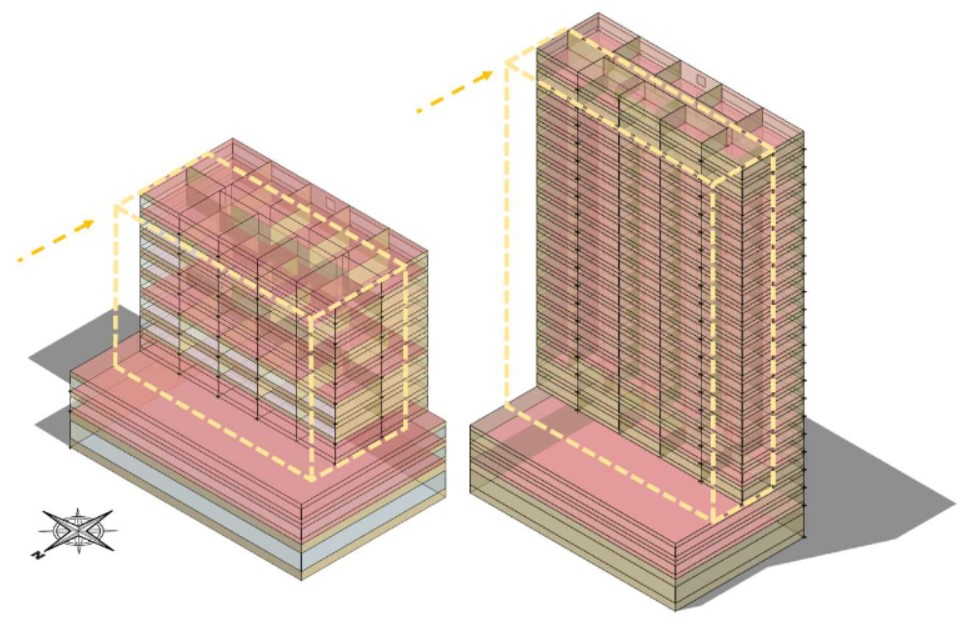
\includegraphics[width=1.0\textwidth]{figures/fig22-modelos.jpg}
        \begin{flushleft}
            \par \small Fonte: autor, (2019).
        \end{flushleft}
        \label{fig:figure22}
    \end{figure}